\documentclass[11pt,a4paper]{article}

% ---- Packages ----
\usepackage[margin=2cm]{geometry}
\usepackage{graphicx}
\usepackage{booktabs}
\usepackage{xcolor}
\usepackage{listings}
\usepackage{tikz}
\usetikzlibrary{positioning}
\usepackage{pgfplots}
\pgfplotsset{compat=1.18}
\usepackage{amsmath}
\usepackage{hyperref}
\usepackage{fancyhdr}
\usepackage{titlesec}
\usepackage{mdframed}
\usepackage{multicol}
\usepackage{enumitem}
\usepackage{tcolorbox}
\tcbuselibrary{skins,breakable}

% ---- Colors ----
\definecolor{primary}{RGB}{0,82,155}
\definecolor{accent}{RGB}{0,153,204}
\definecolor{lightgray}{RGB}{245,245,245}
\definecolor{codebg}{RGB}{30,30,30}
\definecolor{codegreen}{RGB}{106,153,85}
\definecolor{codeyellow}{RGB}{220,220,170}
\definecolor{codeblue}{RGB}{86,156,214}
\definecolor{darkred}{RGB}{180,30,30}

% ---- Section formatting ----
\titleformat{\section}{\large\bfseries\color{primary}}{}{0em}{}[\color{accent}\hrule]
\titleformat{\subsection}{\normalsize\bfseries\color{primary}}{}{0em}{}

% ---- Code listing style ----
\lstdefinestyle{cstyle}{
  backgroundcolor=\color{codebg},
  basicstyle=\ttfamily\footnotesize\color{white},
  keywordstyle=\color{codeblue}\bfseries,
  commentstyle=\color{codegreen},
  stringstyle=\color{codeyellow},
  breaklines=true,
  frame=single,
  rulecolor=\color{accent},
  framesep=4pt,
  xleftmargin=6pt,
  language=C,
  morekeywords={MPI_Exscan,MPI_Bcast,MPI_Reduce,MPI_Barrier,MPI_Wtime,MPI_Abort,MPI_UNSIGNED_LONG_LONG,MPI_LONG_LONG,MPI_SUM,MPI_COMM_WORLD}
}

% ---- Header / Footer ----
\pagestyle{fancy}
\fancyhf{}
\fancyhead[L]{\small\color{primary}\textbf{MPI Distributed Text Search}}
\fancyhead[R]{\small\color{primary}Performance Analysis Report}
\fancyfoot[C]{\small\thepage}
\renewcommand{\headrulewidth}{0.4pt}

% ---- tcolorbox styles ----
\tcbset{
  challenge/.style={
    colback=blue!5, colframe=primary,
    fonttitle=\bfseries\small, title=#1,
    left=4pt, right=4pt, top=3pt, bottom=3pt,
    boxrule=0.8pt
  },
  trick/.style={
    colback=orange!8, colframe=orange!70!black,
    fonttitle=\bfseries\small, title=#1,
    left=4pt, right=4pt, top=3pt, bottom=3pt,
    boxrule=0.8pt
  }
}

% ================================================================
\begin{document}

% ================================================================
%  TITLE PAGE
% ================================================================
\begin{titlepage}
% \begin{tikzpicture}[remember picture, overlay]
%   % Top bar
%   \fill[primary] (current page.north west) rectangle +(\paperwidth, -3.5cm);
%   % Bottom bar
%   \fill[accent] (current page.south west) rectangle +(\paperwidth, 1.2cm);
%   % Decorative circle
%   \fill[accent!40] (current page.north east) +(-3cm,-3cm) circle (4cm);
%   \fill[primary!80] (current page.north east) +(-2cm,-2cm) circle (2.5cm);
% \end{tikzpicture}

\vspace*{1.5cm}
\begin{center}
  {\color{black}\fontsize{22}{28}\selectfont\bfseries MPI Distributed Text Search}\\[0.4cm]
  {\color{white!80}\large Performance Analysis Report}\\[0.3cm]
  {\color{white!60}\normalsize Searching a 10\,GB text file with Boyer--Moore--Horspool}
\end{center}

\vspace{3.5cm}

\begin{center}
\begin{tcolorbox}[width=0.75\textwidth,
  colback=white, colframe=primary,
  boxrule=1pt, arc=6pt,
  title={\color{white}\bfseries Team Members},
  colbacktitle=primary]
  \centering
  \textbf{Mahmoud Atef Mahmoud Abdelaziz}\\[3pt]
  \textbf{Mohamed Alaa Ahmed}\\[3pt]
  \textbf{Abdelrahman Osama Adel}
\end{tcolorbox}
\end{center}

\vspace{1.2cm}

\begin{center}
\begin{tcolorbox}[width=0.75\textwidth,
  colback=lightgray, colframe=accent,
  boxrule=0.8pt, arc=6pt]
  \centering
  \small Under the supervision of\\[4pt]
  \textbf{Prof.\ Dr.\ Sabah Saad}\quad\&\quad\textbf{Eng.\ Mohamed AbdelMageed}\\[4pt]
  High Performance Computing \quad|\quad 2026
\end{tcolorbox}
\end{center}

\vfill
\begin{center}
  \color{white}\small April 2025
\end{center}
\end{titlepage}

% ================================================================
%  PAGE 2 — TASK + ALGORITHM + CHALLENGES
% ================================================================
\section{Task Description}

The goal is to search for a user-defined token (substring) inside a \textbf{10\,GB plain-text file} as fast as possible using \textbf{MPI parallelism}.
Each MPI rank owns a contiguous byte range of the file, scans it independently, and produces a result file listing every match as \texttt{(row, column, byte-offset)}.
A serial baseline (single process, same code) is used for correctness checks and speedup measurement.

\vspace{0.4cm}

\begin{multicols}{2}
\subsection{Algorithm: Boyer--Moore--Horspool (BMH)}

BMH is a practical single-pattern string-search algorithm that preprocesses a \textit{bad-character skip table} from the pattern.
During search it compares from the \emph{right} end of the window and, on a mismatch, skips forward by the table value — often skipping several characters at once.

\begin{center}
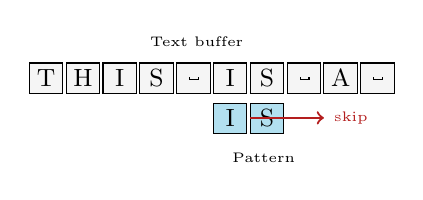
\begin{tikzpicture}[font=\small, scale=0.85]
  % Text buffer
  \foreach \i/\c in {0/T,1/H,2/I,3/S,4/\textvisiblespace,5/I,6/S,7/\textvisiblespace,8/A,9/\textvisiblespace}{
    \draw[fill=lightgray] (\i*0.55,0) rectangle (\i*0.55+0.5,0.45);
    \node at (\i*0.55+0.25, 0.22) {\c};
  }
  % Pattern aligned
  \foreach \i/\c in {0/I,1/S}{
    \draw[fill=accent!30] (\i*0.55+2.75,-.6) rectangle (\i*0.55+3.25,-.15);
    \node at (\i*0.55+3.0, -.37) {\c};
  }
  \draw[->,thick,darkred] (3.3,-0.37) -- (4.4,-0.37) node[right]{\tiny skip};
  \node[above] at (2.5, 0.55) {\tiny Text buffer};
  \node[below] at (3.5,-0.75) {\tiny Pattern};
\end{tikzpicture}
\end{center}

\textbf{Preprocessing} (done once per rank):
\begin{lstlisting}[style=cstyle]
void bmh_preprocess(const char *token,
    int tlen, int skip[BMH_ALPHA]) {
  for (int i=0;i<BMH_ALPHA;i++) skip[i]=tlen;
  for (int i=0;i<tlen-1;i++)
    skip[(unsigned char)token[i]] = tlen-1-i;
}
\end{lstlisting}

\columnbreak

\subsection{Single-Pass Design}

Rather than two sequential file reads, each rank performs \textbf{one heavy pass}:

\begin{enumerate}[leftmargin=*,nosep,label=\textcolor{primary}{\arabic*.}]
  \item Read owned chunk (+ overlap bytes)
  \item Count newlines \& track column position
  \item Collect \texttt{LocalMatch} records in a \textit{dynamic array}
  \item After the pass: \texttt{MPI\_Exscan} converts local rows to global rows
  \item Deferred write phase: dump matches to per-rank result file
\end{enumerate}

\begin{center}
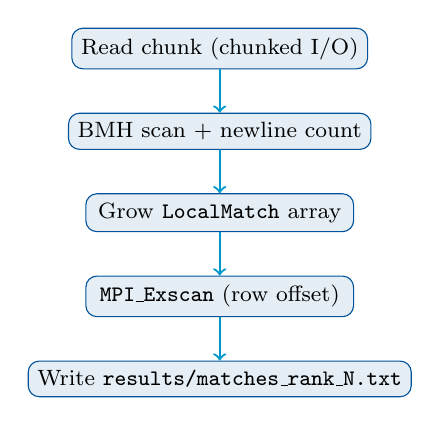
\begin{tikzpicture}[font=\footnotesize, node distance=0.55cm, auto]
  \tikzstyle{box}=[rectangle,rounded corners,draw=primary,fill=primary!10,
                   minimum width=3.4cm, minimum height=0.45cm, align=center]
  \tikzstyle{arr}=[->,thick,color=accent]
  \node[box](a){Read chunk (chunked I/O)};
  \node[box,below=of a](b){BMH scan + newline count};
  \node[box,below=of b](c){Grow \texttt{LocalMatch} array};
  \node[box,below=of c](d){\texttt{MPI\_Exscan} (row offset)};
  \node[box,below=of d](e){Write \texttt{results/matches\_rank\_N.txt}};
  \draw[arr](a)--(b); \draw[arr](b)--(c);
  \draw[arr](c)--(d); \draw[arr](d)--(e);
\end{tikzpicture}
\end{center}
\end{multicols}

\vspace{0.3cm}
\section{Challenges \& How They Were Solved}

\begin{tcolorbox}[challenge={Challenge 1 — Which string-matching algorithm?}]
\textbf{Problem:} Naïve search is $O(n \cdot m)$; on 10\,GB this is too slow even serially.\\
\textbf{Solution:} \textbf{Boyer–Moore–Horspool} — sub-linear average case, simple bad-character table (256 entries), cache-friendly right-to-left comparison. For a pattern of length $m$, the skip table is built in $O(m)$ and each search step is $O(m)$ worst-case but \emph{$O(n/m)$ on average}.
\end{tcolorbox}

\vspace{0.25cm}

\begin{tcolorbox}[challenge={Challenge 2 — File with no spaces (dense text)}]
\textbf{Problem:} If the file contains no whitespace, \texttt{--whole-word} mode cannot rely on spaces as delimiters, and the skip table rarely gets to skip many bytes.\\
\textbf{Solution:} The word-boundary check uses \texttt{isalnum()} and underscore, not just whitespace.
For no-space files, \texttt{--whole-word} is simply disabled (default) so the skip table still fires on any mismatch of the pattern's last character.
\end{tcolorbox}

\vspace{0.25cm}

\begin{tcolorbox}[challenge={Challenge 3 — Token split across two rank boundaries}]
\textbf{Problem:} If a token of length $m$ straddles the boundary between rank $k$ and rank $k{+}1$, neither rank would normally find it.\\
\textbf{Solution:} Each rank reads \textbf{$(m-1)$ extra bytes} to the right of its owned range (the \emph{overlap}), but only \emph{reports} matches whose byte offset falls within its strict owned range. This is computed in \texttt{collect\_matches\_single\_pass}:
\begin{lstlisting}[style=cstyle]
int overlap = (tlen > 1) ? (tlen - 1) : 0;
long long right_extra = overlap;
// ...
if (off >= cur && off < cur + own_len &&
    off >= my_start && off < my_end)   // strictly owned
    // record match
\end{lstlisting}
Every cross-boundary token is therefore seen by exactly one rank (the one that owns its starting byte), with \textbf{no duplicates and no misses}.
\end{tcolorbox}

% ================================================================
%  PAGE 3 — IMPLEMENTATION TRICKS
% ================================================================
\newpage
\section{Implementation Tricks}

\begin{multicols}{2}

\begin{tcolorbox}[trick={Trick 1 — Dynamic growing match array}]
Matches are stored in a heap-allocated \texttt{LocalMatch} array that doubles on overflow (\texttt{realloc}). This avoids a fixed-size limit without a costly pre-count pass.
\begin{lstlisting}[style=cstyle]
if (local_match_count==array_capacity){
  size_t nc = array_capacity * 2;
  LocalMatch *nx = realloc(matches,
      nc * sizeof(LocalMatch));
  matches = nx;
  array_capacity = nc;
}
\end{lstlisting}
\end{tcolorbox}

\vspace{0.3cm}

\begin{tcolorbox}[trick={Trick 2 — MPI\_Exscan for global line numbers}]
\texttt{MPI\_Exscan} computes the \emph{exclusive prefix sum} of local newline counts, giving each rank its global line offset with a single collective call — no explicit loop over ranks.
\begin{lstlisting}[style=cstyle]
MPI_Exscan(&chunk_newline_count,
           &global_line_offset,
           1, MPI_UNSIGNED_LONG_LONG,
           MPI_SUM, MPI_COMM_WORLD);
if (rank == 0) global_line_offset = 0;
\end{lstlisting}
Rank 0's exscan result is undefined by the MPI standard, so it is explicitly reset to 0.
\end{tcolorbox}

\columnbreak

\begin{tcolorbox}[trick={Trick 3 — Chunked I/O to control memory}]
Each rank reads its byte range in configurable \texttt{chunk\_mb} slices. This prevents mapping the entire 10\,GB file into RAM even for a single rank, enabling the program to run on memory-constrained nodes.
\end{tcolorbox}

\vspace{0.3cm}

\begin{tcolorbox}[trick={Trick 4 — Left-overlap read for boundary safety}]
When \texttt{cur > 0} the rank reads \textbf{1 extra byte to the left} to allow the whole-word boundary check to inspect the character immediately before the owned region without additional IPC.
\begin{lstlisting}[style=cstyle]
long long left_extra = (cur > 0) ? 1 : 0;
read_start = cur - left_extra;
// owned_start_idx = left_extra (skip in output)
\end{lstlisting}
\end{tcolorbox}

\vspace{0.3cm}

\begin{tcolorbox}[trick={Trick 5 — Deferred write / compute-write overlap}]
All match metadata is buffered in RAM during the search pass, then flushed to disk in a separate write phase \emph{after} \texttt{MPI\_Exscan}. This means disk writes happen once, in order, with correct global line numbers — no seeks or re-opens.
\end{tcolorbox}

\end{multicols}

% ================================================================
%  PAGE 4 — PERFORMANCE RESULTS
% ================================================================
\newpage
\section{Performance Results}

\subsection{Experimental Setup}

\begin{center}
\begin{tabular}{ll}
\toprule
\textbf{Parameter} & \textbf{Value} \\
\midrule
File size & 10\,GB randomly generated text \\
Search token & fixed keyword \\
Chunk size & 64\,MB per rank per iteration \\
Repeats per condition & 5 (average + std reported) \\
Serial baseline & \texttt{--impl serial}, \texttt{np=1} \\
MPI conditions & \texttt{np} $\in \{2,4,8\}$ \\
\bottomrule
\end{tabular}
\end{center}

\vspace{0.4cm}
\subsection{Raw Timing Data}

\begin{center}
\resizebox{\textwidth}{!}{
\begin{tabular}{ccccccc}
\toprule
\textbf{np} & \textbf{Run 1 (s)} & \textbf{Run 2 (s)} & \textbf{Run 3 (s)} & \textbf{Run 4 (s)} & \textbf{Run 5 (s)} & \textbf{Avg $\pm$ Std (s)} \\
\midrule
Serial & 20.92 & 21.12 & 21.37 & 20.91 & 20.86 & $21.03 \pm 0.21$ \\
2      & 17.05 & 21.61 & 16.29 & 16.14 & 16.11 & $17.44 \pm 2.36$ \\
4      & 8.72  & 8.54  & 9.13  & 8.60  & 7.60  & $8.52 \pm 0.56$ \\
8      & 7.10  & 6.63  & 7.61  & 7.10  & 6.27  & $6.94 \pm 0.51$ \\
\bottomrule
\end{tabular}
}
\end{center}

\vspace{0.4cm}
\subsection{Speedup vs Number of Processes}

\begin{center}
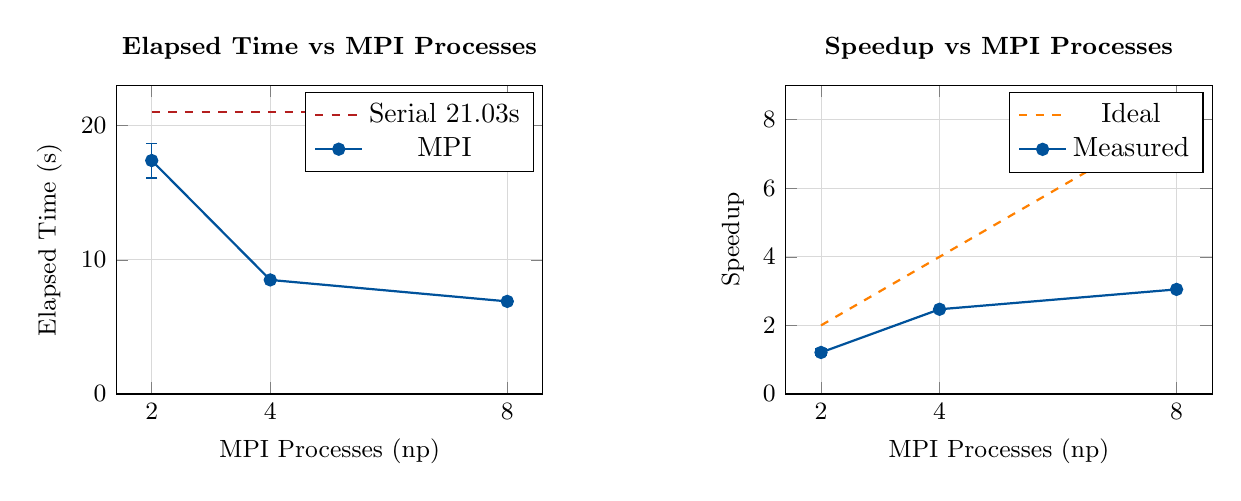
\begin{tikzpicture}
\begin{axis}[
  width=7cm, height=5.5cm,
  title={\small\textbf{Elapsed Time vs MPI Processes}},
  xlabel={MPI Processes (np)},
  ylabel={Elapsed Time (s)},
  xtick={2,4,8},
  ymin=0, ymax=23,
  grid=both, grid style={line width=0.3pt,draw=gray!30},
  tick label style={font=\small},
  label style={font=\small},
  at={(0,0)},
]
  \addplot[dashed, thick, color=darkred, domain=2:8] {21.03};
  \addlegendentry{Serial 21.03s}
  \addplot[mark=*, thick, color=primary, error bars/.cd,
    y dir=both, y explicit]
    coordinates {
      (2,17.4) +- (0,1.3)
      (4,8.5)  +- (0,0.2)
      (8,6.9)  +- (0,0.2)
    };
  \addlegendentry{MPI}
\end{axis}
\begin{axis}[
  width=7cm, height=5.5cm,
  title={\small\textbf{Speedup vs MPI Processes}},
  xlabel={MPI Processes (np)},
  ylabel={Speedup},
  xtick={2,4,8},
  ymin=0, ymax=9,
  grid=both, grid style={line width=0.3pt,draw=gray!30},
  tick label style={font=\small},
  label style={font=\small},
  at={(8.5cm,0)},
]
  \addplot[dashed, thick, color=orange, domain=2:8] {x};
  \addlegendentry{Ideal}
  \addplot[mark=*, thick, color=primary, error bars/.cd,
    y dir=both, y explicit]
    coordinates {
      (2, 1.21) +- (0,0.10)
      (4, 2.47) +- (0,0.06)
      (8, 3.05) +- (0,0.09)
    };
  \addlegendentry{Measured}
\end{axis}
\end{tikzpicture}
\end{center}

\vspace{0.3cm}

\begin{tcolorbox}[colback=lightgray,colframe=primary,boxrule=0.8pt]
\small
\textbf{Key observations:}
\begin{itemize}[nosep,leftmargin=*]
  \item \textbf{np=2} gives only $\approx1.2\times$ speedup with high variance — I/O bandwidth is the bottleneck at low parallelism; all ranks contend on the same disk.
  \item \textbf{np=4} reaches $\approx2.5\times$ — a good balance between compute parallelism and I/O contention.
  \item \textbf{np=8} plateaus at $\approx3.0\times$ — sub-linear because 8 ranks saturate disk bandwidth; the bottleneck shifts from CPU to storage I/O.
  \item The gap from ideal (dashed orange) reflects \textbf{Amdahl's Law}: serial I/O setup, MPI collectives (\texttt{Exscan}, \texttt{Barrier}), and disk saturation all contribute to the overhead fraction.
\end{itemize}
\end{tcolorbox}

% ================================================================
%  PAGE 5 — ANALYSIS + CONCLUSION
% ================================================================
\newpage
\section{Analysis \& Discussion}

\begin{multicols}{2}
\subsection{Amdahl's Law Fit \& I/O Saturation}

Amdahl's Law predicts the maximum theoretical speedup $S(p)$ given a strictly serial fraction $f$ of the execution time:
\[
  S(p) = \frac{1}{f + \frac{1-f}{p}}
\]
Fitting the formula to our measured np=4 speedup ($\approx2.47\times$) gives a calculated serial fraction of $f \approx 0.20$. This indicates that approximately \textbf{20\,\%} of the program's execution time consists of inherently serial overhead (OS setup, MPI initialization, and \texttt{MPI\_Exscan} sync).

However, applying $f \approx 0.20$ to np=8 predicts a theoretical speedup of $3.33\times$. Our measured speedup at np=8 plateaus lower, at $3.05\times$. This deviation from Amdahl's ideal curve proves that a secondary bottleneck---hardware disk I/O saturation---is introduced. The storage drive physically cannot serve 8 concurrent read requests without significant context switching, shifting the primary bottleneck away from CPU limits entirely onto storage bandwidth.

\begin{center}
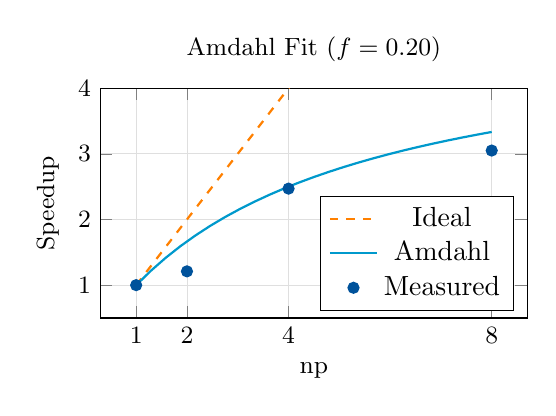
\begin{tikzpicture}
\begin{axis}[
  width=7cm, height=4.5cm,
  xlabel={np}, ylabel={Speedup},
  xtick={1,2,4,8},
  ymin=0.5, ymax=4,
  grid=both, grid style={line width=0.3pt,draw=gray!25},
  tick label style={font=\small},
  label style={font=\small},
  title={\small Amdahl Fit ($f=0.20$)},
  legend pos=south east
]
  \addplot[dashed,orange,domain=1:8,thick]{x};
  \addlegendentry{Ideal}
  % Updated Amdahl curve formula: f=0.20, (1-f)=0.80
  \addplot[domain=1:8,thick,color=accent]{1/(0.20+0.80/x)};
  \addlegendentry{Amdahl}
  \addplot[only marks,mark=*,color=primary]
    coordinates{(1,1)(2,1.21)(4,2.47)(8,3.05)};
  \addlegendentry{Measured}
\end{axis}
\end{tikzpicture}
\end{center}
\columnbreak

\subsection{Bottleneck: Disk I/O}

The dominant bottleneck is disk bandwidth, not CPU. Evidence:
\begin{enumerate}[nosep,leftmargin=*]
  \item Speedup flattens sharply from np=4 to np=8 even though the CPU load is lower.
  \item High variance at np=2 (std=1.3s) indicates contention on random I/O scheduling.
  \item The BMH skip rate on 10\,GB English-like text is high (few false matches), so CPU time is low relative to I/O.
\end{enumerate}

\subsection{Possible Improvements}

\begin{itemize}[nosep,leftmargin=*,label=\textcolor{accent}{$\triangleright$}]
  \item \textbf{Memory-mapped I/O} (\texttt{mmap}) to let the OS pipeline reads.
  \item \textbf{Async I/O} (POSIX AIO or \texttt{io\_uring}) to overlap reading with searching.
  \item \textbf{SSD / NVMe} storage to increase bandwidth ceiling.
  \item \textbf{OpenMP} within each rank for multi-threaded BMH on each chunk.
  \item \textbf{MPI-IO} (\texttt{MPI\_File\_read\_at\_all}) for collective I/O optimisation.
\end{itemize}

\end{multicols}

\vspace{0.4cm}


% ================================================================
%  INFRASTRUCTURE & CONTAINERIZATION
% ================================================================
\section{Infrastructure \& Containerization}

To ensure reproducibility and simulate a realistic High-Performance Computing (HPC) environment on a single host machine, the entire MPI cluster was containerized using Docker. 

\subsection{Node Configuration (Dockerfile)}
The custom Docker image is based on Ubuntu 24.04 and installs the essential HPC stack: GCC, OpenMPI, and Python for benchmarking. A critical challenge in containerized MPI is inter-node communication. MPI relies on SSH to spawn processes on remote workers. To solve this, the \texttt{Dockerfile} automates a \textbf{passwordless SSH environment}: it generates RSA keys, populates \texttt{authorized\_keys}, and explicitly disables \texttt{StrictHostKeyChecking}. This prevents the MPI runtime from hanging on user-interaction prompts during initial connection.

\subsection{Cluster Topology (Docker Compose)}
The cluster is orchestrated via \texttt{docker-compose.yml}, defining a \texttt{master} node and scalable \texttt{worker} nodes. Two key architectural design patterns were implemented:

\begin{tcolorbox}[width=\textwidth, colback=lightgray, colframe=primary, boxrule=0.8pt, arc=4pt]
\small
\begin{itemize}[leftmargin=*,nosep]
  \item \textbf{Dual-Network Isolation:} The cluster utilizes two distinct Docker bridge networks. The \texttt{frontend\_net} allows user interaction with the \texttt{mpi-master}. Meanwhile, the \texttt{compute\_net} is configured as \texttt{internal: true}. Worker nodes are isolated entirely within this internal network, mirroring the secure, dedicated backend switch topologies of real supercomputers.
  \item \textbf{Simulated Shared Storage (NFS):} Both master and worker containers mount the host's directory as a volume (\texttt{./:/app}). This mimics a shared Network File System (NFS), ensuring all MPI ranks have immediate, unified access to the 10\,GB dataset and can write to the isolated \texttt{results/} directory without requiring SCP file transfers.
\end{itemize}
\end{tcolorbox}
\vspace{0.4cm}
\section{Conclusion}

This project demonstrates a scalable, single-pass MPI distributed text search over a 10\,GB file.
Key engineering decisions — \textbf{BMH} for fast pattern skipping, \textbf{overlap bytes} for cross-boundary correctness, \textbf{dynamic match arrays} for memory safety, and \textbf{\texttt{MPI\_Exscan}} for correct global line numbering — combine into a clean and efficient implementation.
Measured speedups of $1.2\times$, $2.5\times$, $3.0\times$ for np $=2,4,8$ are consistent with an I/O-bound workload; further gains require faster storage or asynchronous I/O, not more MPI ranks.

\vspace{0.5cm}

\vspace{0.4cm}
\section{Task Distribution}

\begin{center}
\begin{tcolorbox}[width=0.95\textwidth,
  colback=lightgray, colframe=primary,
  boxrule=0.8pt, arc=4pt,
  title={\color{white}\bfseries Team Workload Distribution},colbacktitle=primary]
\centering
\small
\renewcommand{\arraystretch}{1.4}
\begin{tabular}{p{3.5cm} p{10cm}}
\toprule
\textbf{Team Member} & \textbf{Assigned Responsibilities} \\
\midrule
\textbf{Mohamed Alaa} & \textbf{Project Initialization \& Data Generation:} \newline
$\triangleright$ Initialized the C project structure and build system (\texttt{Makefile}). \newline
$\triangleright$ Developed the 10\,GB text corpus generator (\texttt{gen\_text}). \newline
$\triangleright$ Established the serial baseline implementation for correctness testing. \\
\midrule
\textbf{Mahmoud Atef} & \textbf{Core Search Algorithm \& MPI Architecture:} \newline
$\triangleright$ Implemented the Boyer--Moore--Horspool (BMH) search logic. \newline
$\triangleright$ Designed the Single-Pass memory management and overlap boundary checks. \newline
$\triangleright$ Developed the \texttt{MPI\_Exscan} integration for global row calculations. \\
\midrule
\textbf{Abdelrahman Osama} & \textbf{Infrastructure, Testing \& Visualization:} \newline
$\triangleright$ Engineered the containerized MPI cluster using Docker (\texttt{docker-compose.yml}). \newline
$\triangleright$ Created the automated benchmarking pipeline (\texttt{run\_experiments.sh}). \newline
$\triangleright$ Developed the Python data parsing and Matplotlib visualization scripts. \\
\bottomrule
\end{tabular}
\end{tcolorbox}
\end{center}

\end{document}